\documentclass[twocolumn,twoside,10pt,a4paper]{article}

\usepackage[english]{babel}  % portuguese
\usepackage{graphicx}           % images: .png or .pdf w/ pdflatex; .eps w/ latex

%% For iso-8859-1 (latin1), comment next line and uncomment the second line
\usepackage[utf8]{inputenc}

\usepackage{times}              % PS fonts
\usepackage[T1]{fontenc}        % T1 fonts
%\usepackage{lastpage}           % to have lastpage in headers
\usepackage{url}                % urls

% geometry package
\usepackage[outer=20mm,inner=30mm,vmargin=20mm,includehead,includefoot,headheight=15pt]{geometry}

%% space between columns
\columnsep 10mm

% avoid widows and orphans
\clubpenalty=300
\widowpenalty=300

\usepackage{listings}
\lstdefinestyle{xml}{
	language=XML,
	extendedchars=true,
	inputencoding=latin1,
	tabsize=4,
	showstringspaces=false,
	basicstyle=\scriptsize,
	keywordstyle=\ttfamily\color{blue},
	stringstyle=\ttfamily\color{orange},
	identifierstyle=\ttfamily,
	commentstyle=\ttfamily\color{darkred},
	morecomment=[s][\ttfamily\color{javadoc}]{/**}{*/},
	numbers=left
}

\usepackage[pdftex]{hyperref}
\hypersetup{%
    a4paper = true,              % use A4 paper
    bookmarks = true,            % make bookmarks
    colorlinks = true,           % false: boxed links; true: colored links
    pdffitwindow = false,        % page fit to window when opened
    pdfpagemode = UseNone,       % do not show bookmarks
    pdfpagelayout = SinglePage,  % displays a single page
    pdfpagetransition = Replace, % page transition
    linkcolor=blue,              % hyperlink colors
    urlcolor=blue,
    citecolor=blue,
    anchorcolor=green
}

\usepackage{indentfirst}       % indent also 1st paragraph

\pagestyle{myheadings}         % Option to put page headers
\markboth{{\small\it xml2json - An XSLT approach}}
{{\small\it Group 08, \today}}

%\hyphenation{}                  % explicit hyphenation

% entities
\newcommand{\class}[1]{{\normalfont\slshape #1\/}}

\title{xml2json\\\footnotesize{An XSLT approach}}

\author{João Gradim\\
\small Faculdade de Engenharia da Universidade do Porto,\\[-0.8ex]
\small R.\ Dr.\ Roberto Frias, 4200-465 Porto\\[-0.8ex]
\small \texttt{ei05030@fe.up.pt}\\
\and
Nuno Polónia\\
\small Faculdade de Engenharia da Universidade do Porto,\\[-0.8ex]
\small R.\ Dr.\ Roberto Frias, 4200-465 Porto\\[-0.8ex]
\small \texttt{ei05037@fe.up.pt}
}

\date{\today}

\begin{document}

\maketitle
\thispagestyle{plain}

\begin{abstract}

JSON is a lightweight data-interchange format, used often for serialization and data transmission across network connections, as an alternative to XML\cite{json_format}.\\
This projects aims to provide an XSL stylesheet that is able to transform any XML document (as long as it is well-formed) to a JSON representation, while maintaining the original document structure.

\end{abstract}
\section{Introduction}\label{sec:intro}


JSON was specified by Douglas Crockford in the RFC 4627 in July of 2006\cite{rfc4627}. It is an open, language-independent standard, based on a subset of the Javascript Language.\\
It's simplicity and lightweightness turned it into the most commonly used format in serialization and data transmission for web apps. While XML is a more generic language which uses more syntactically complex structures, JSON relies only on two structures, a collection of name/value pairs and an ordered list of values\cite{json_format}, to represent objects.
With the crescent growth of websites functionalities and the need of faster response times, web developers rely on JSON for communication. Most of the API's available have both XML and JSON output. But some API's like the MusicBrainz or the Last.fm, only have output in XML.\\
The purpose of this work is to create a conversion stylesheet from any well formed XML document to JSON without losing any of the information or structure of the data contained in the XML document. In the first chapter of this document the conditions of the XML documents accepted by the XSL stylesheet will be specified. In the second chapter we'll talk about the characteristics of the generated JSON output. In the third chapter the details of the XSL stylesheet are designated.

\section{Valid Source Dialects}\label{sec:valid-source-dialects}

This project supports virtually every existing XML document, as it does not require any specific elements, attributes or document structure. As long as the source document is well-formed, the stylesheet is able to produce a valid JSON representation of the aforementioned XML document, while maintaining its structure.\\

\section{JSON Output}\label{sec:json-output}

JSON represents an object as an unordered collection of key/value pairs (also known as associative arrays, hashes or dictionaries) and ordered lists of objects or values (also know as arrays, or lists).\\
A well formed XML document has a node that contains (i.e., is an ancestor of) every other node in the document, and is often called the \emph{root node}.\\
As such, the output produced by this stylesheet creates an object with a single key corresponding to the name of the root node. This key maps to an object that holds every other node of the document, preserving the structure of the original document.\\
Every element in the original document is represented as a key that maps to an object: this object contains every attribute, child nodes and textual content for the element.

\subsection{Attributes}

XML attribute nodes are represented as key/value pairs: the key is a string built by concatenating an \verb!@! with the attribute's name. This key maps to a value (either a string or a number) representing the value of that attribute.\\

\subsection{Textual Content}

XML text nodes are mapped to the \verb!"$text"! property of an object. If an element has multiple children text nodes, an index is appended to this key, creating as many keys as text nodes present: \verb!"$text1"!, \verb!"$text2"!, etc.\\

\section{XSLT Stylesheet}\label{sec:xslt-stylesheet}

The transformation starts out by matching the root node and enclosing the whole transformation within a pair of brackets (\verb!{}!). A template is then applied that matches every element in the original document. This template is responsible for transforming an XML element into a JSON object, by opening and closing objects (\verb!{}!) and arrays (\verb![]!), and by separating different elements. During this process, the attributes are processed in order to add them to the element declaration. After processing the element's attributes, and text nodes, this template is applied recursively to the element's child nodes so that nested elements are accounted for.

\subsection{Attribute values and text nodes}

Attribute values and text nodes are processed by a series of templates that ensure their validity and correct representation\cite{json_format}. An initial test is performed in order to determine if said value is a number: if true, the value is printed \textit{as is}; otherwise, the value is regarded as a string: the value in enclosed between doubles quotes and their contents are analyzed in order to escape invalid characters (backslash and double quotes).

\subsection{Arrays}
An XML element whose children all have the same name would generate a JSON object with multiple equal keys. As JSON does not allow repeated keys in objects (the only valid key/value mapping would be the last one to be defined), these elements must be represented as an array of JSON objects. To handle these situations a template is applied, matching only if all the children nodes have the same name and the count of these number is greater than one (example on Fig. \ref{fig:array_xml2json}).

\begin{figure}[h]
\centering
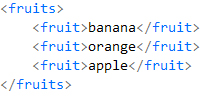
\includegraphics[width=35mm]{images/array_xml.jpg}
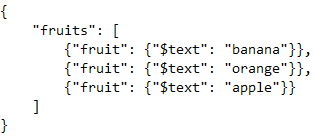
\includegraphics[width=55mm]{images/array_json.jpg}
\caption{Transformation of an array from XML to JSON}
\label{fig:array_xml2json}
\end{figure}


\subsection{Multiple siblings with same name}
There are situations in which there are multiple XML elements in the same level with the same name followed or preceded by siblings with different names. In this case it would be incorrect in terms of structure to map those elements to an array and if those siblings with the same name weren't treated, information would be lost as JSON doesn't allow multiple declarations of same named keys.

In order to avoid the redeclaration of those keys which would lead to the loss of information, an index is appended to the name of the element. This operation mantains the integrity of both the information and structure of the XML document when the transformation is applied (example on Fig. \ref{fig:group_xml2json}).

\begin{figure}[h]
\centering
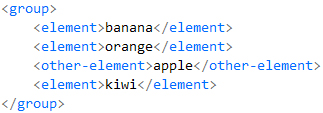
\includegraphics[width=55mm]{images/group_xml.jpg}
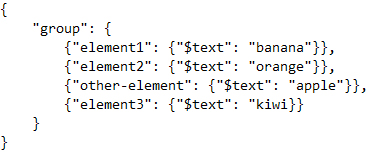
\includegraphics[width=60mm]{images/group_json.jpg}
\caption{Transformation of multiple siblings with the same name from XML to JSON}
\label{fig:group_xml2json}
\end{figure}

\section{Final Remarks}\label{sec:final-remarks}

XSLT proves to be a very capable and efficient tool to manipulate XML documents. It revealed to be an intuitive XML manipulation tool, allowing for a level of abstraction where the only alternative would be to use a specialized parser, that could reveal itself as excessively heavy or prone to failure in face of certain situations.

With the conclusion of this project it can be stated that XML can be effectively represented as a JSON object without any loss of data or document structure (except for node order, which, depending on the implementation of the destiny language, can be lost, as hashes or associative arrays are often unordered, depending on the implementation).

\section{Future Work}\label{sec:future-work}
The next step will be to create a web service which acts as a proxy for API's that only have XML output allowing web developers to have the results from those API's in JSON.



%% auto bibliographic list
\renewcommand{\bibname}{References}
\bibliographystyle{unsrt-pt}
\bibliography{lapd2}

\end{document}

